\section{Busca em árvore binária de busca} \label{cap:3:section:bst}

\subsection{Introdução}

O algoritmo de busca em árvore binária de busca, funciona de modo que, vamos percorrer
a árvore, testando se o nó atual é maior ou menor que o elemento $x$, se for maior, tomamos
o caminho da esquerda, se for menor, tomamos o caminho da direita. Esse algoritmo pode ser implementado
porque a árvore binária de busca é uma estrutura que segue as seguintes proposições:

\begin{align*}
    NODE.PARENT \geq NODE.LEFT \\
    NODE.PARENT \leq NODE.RIGHT
\end{align*}

\subsection{Implementação}

A implementação do algoritmo de busca em árvore binária de busca funciona percorrendo
a árvore de forma organizada com as comparações do nó atual com o elemento $x$.

\begin{lstlisting}[style=CStyle]
Node * search(Node * root, int key) 
{
    if (root == NULL || root->data == key) {
        return root;
    }

    if (key < root->data) {
        return search(root->left, key);
    } else {
        return search(root->right, key);
    }
}
\end{lstlisting}
                    

Seu tempo de execução é na ordem da equação \ref{cap:3:eq:bst}.

\begin{equation} \label{cap:3:eq:bTree}
    T(n) = O(\log n)
\end{equation}

\subsection{Resultados}

Para a implementação, foi obtido o gráfico \ref{cap:3:graph:bst}:

\begin{figure}[h]
    \centering
    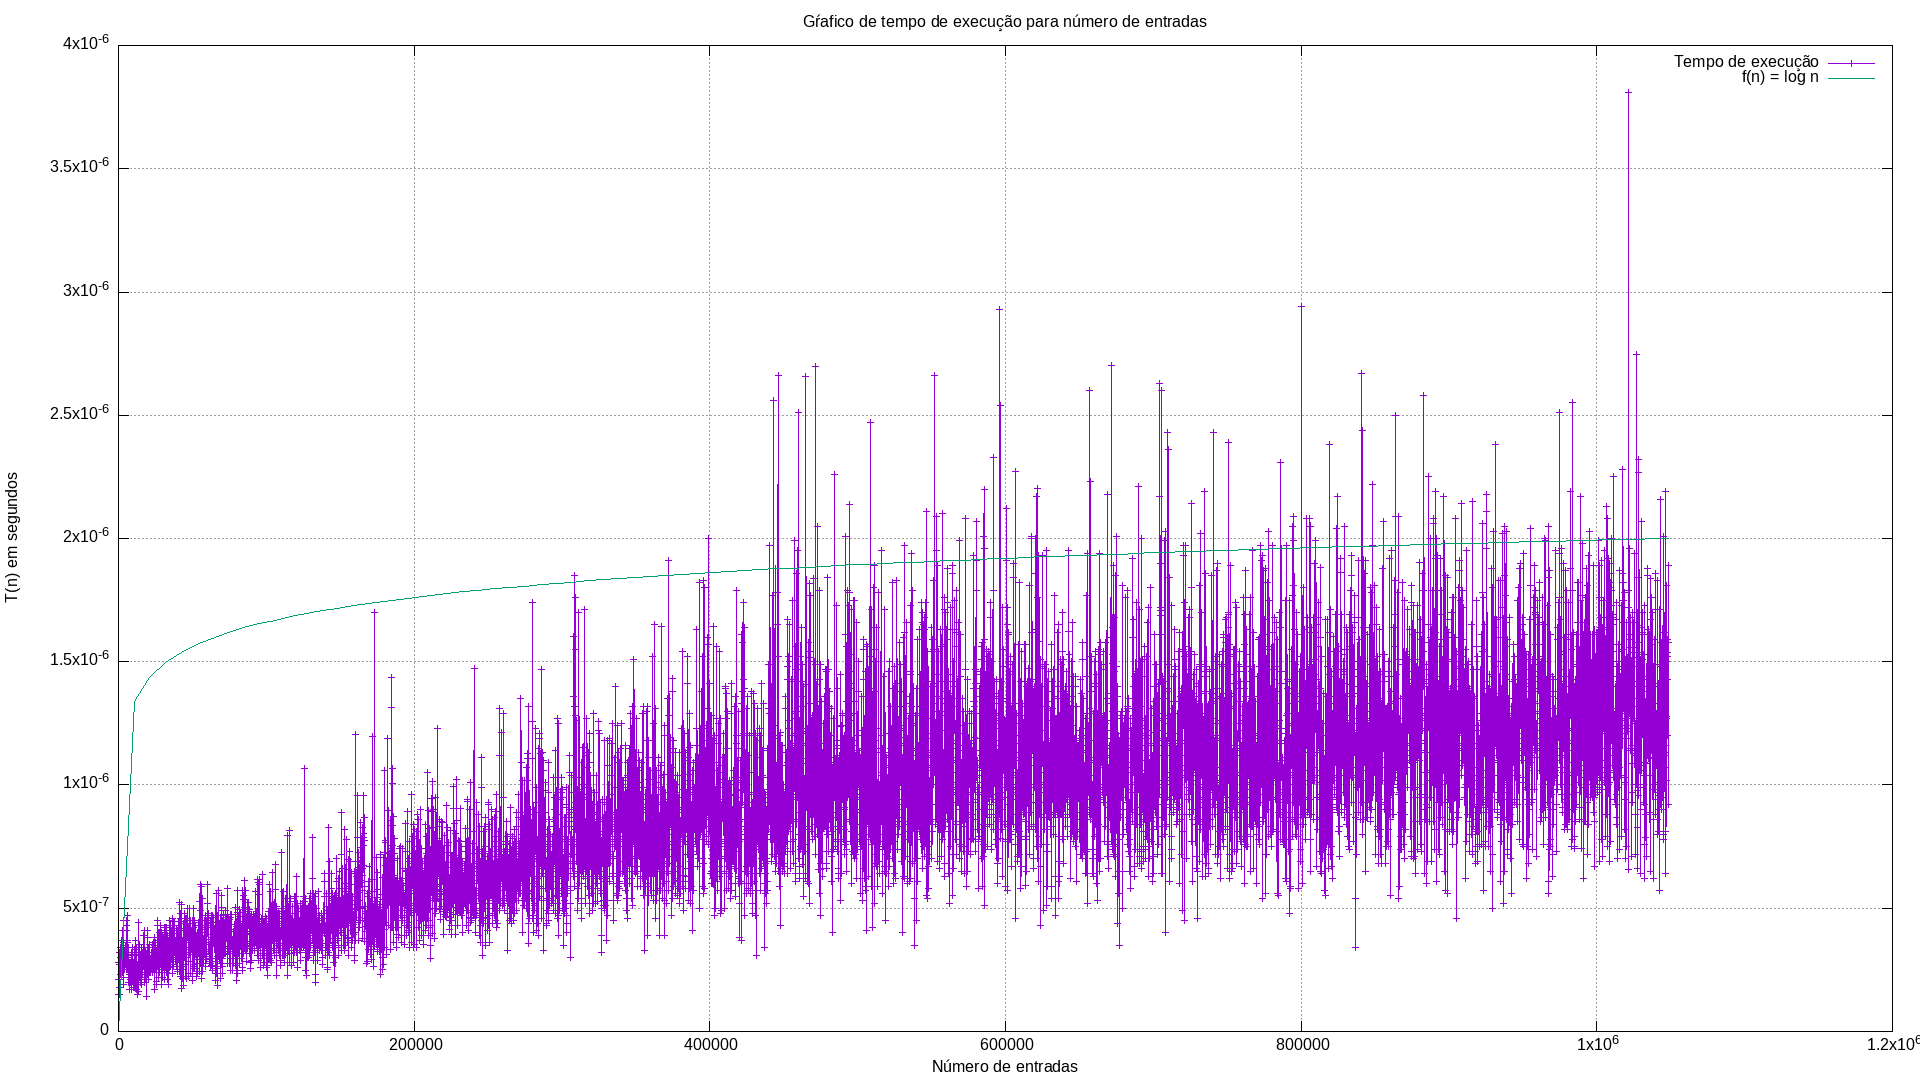
\includegraphics[width=\textwidth]{image/graphics/bst.png}
    \caption{Gráfico com tempo de execução do algoritmo de busca em árvore de busca binária}
    \label{cap:3:graph:bst}
\end{figure}

O gráfico obtido indica que:
